% Resultados y discusión, prueba por prueba. Tablas y figuras generadas por
% python -m analysis.capitulo5 a partir de los lotes (Anexo A).

Este capítulo presenta los resultados de las pruebas de la
Tabla~\ref{tab:experimentos}, en el mismo orden. Para cada prueba se recuerda
qué se esperaba y se compara con lo obtenido; la Tabla~\ref{tab:resumen-pruebas},
al final, las resume. Salvo que se indique otra cosa, las cifras son el promedio
$\pm$ la desviación estándar de 10 semillas, calculadas directamente a partir de
los lotes. Las figuras y tablas de este documento que no indican fuente son de
elaboración propia.

\section{Funciones básicas (pruebas P1 y P2)}
\label{sec:res-basicas}

\textbf{P1, formación de la malla.} Se esperaba que, sin ninguna ayuda, los
nodos se descubrieran y llenaran sus tablas de rutas. A los 30~s de la corrida
con la semilla 1, 152 de los 156 pares de nodos conectados por radio ya tenían
una ruta vigente, es decir, el 97~\% (Figura~\ref{fig:matriz}a). Los cuatro
pares que faltan son pares lejanos, entre el piso 1 y el piso 3: sus OGM deben
cruzar muchos saltos de enlaces con pérdidas, cerca del límite de 6 saltos del
TTL. La prueba se cumple.

\textbf{P2, propagación de un OGM.} Se esperaba que el TTL bajara en uno por
cada salto. En la Figura~\ref{fig:ogm}, las copias del mensaje de G1 llevan ttl
6 al salir de G1, ttl 5 al salir de sus vecinos directos, y ttl 3 y 2 las que ya
fueron reenviadas tres y cuatro veces.
La prueba se cumple.

\section{Tipos de paquete (prueba P3)}
\label{sec:res-tipos}

Se esperaba que ICMP entregara menos que UDP, porque un eco necesita que
lleguen la ida y la vuelta, y que TCP entregara más que UDP, a cambio de más
transmisiones. La Tabla~\ref{tab:cap5-tipos} lo confirma con 6 flujos entre
usuarios en el despliegue de referencia.

% Generado por python -m analysis.capitulo5 (no editar a mano).
\begin{table}[htbp!]
    \centering
    \caption{Entrega según el tipo de paquete en el despliegue de referencia}
    \label{tab:cap5-tipos}
    \footnotesize
    \setlength{\tabcolsep}{3pt}
    \begin{tabular}{|>{\raggedright\arraybackslash\hspace{0pt}}p{4.3cm}|>{\raggedright\arraybackslash\hspace{0pt}}p{2.0cm}|>{\raggedright\arraybackslash\hspace{0pt}}p{2.2cm}|>{\raggedright\arraybackslash\hspace{0pt}}p{1.6cm}|>{\raggedright\arraybackslash\hspace{0pt}}p{1.9cm}|>{\raggedright\arraybackslash\hspace{0pt}}p{1.9cm}|}
        \hline
        \textbf{Tipo de paquete} & \textbf{Entrega de datos} & \textbf{Transmisiones por paquete} & \textbf{Saltos} & \textbf{Perdidos por el radio} & \textbf{Perdidos sin ruta} \\
        \hline
        UDP (sin confirmación) & 0.772 $\pm$ 0.061 & 7.46 $\pm$ 1.96 & 3.91 $\pm$ 0.74 & 0.155 $\pm$ 0.048 & 0.053 $\pm$ 0.035 \\
        \hline
        ICMP (eco: ida y vuelta) & 0.646 $\pm$ 0.082 & 11.83 $\pm$ 2.67 & 3.85 $\pm$ 0.72 & 0.256 $\pm$ 0.060 & 0.079 $\pm$ 0.024 \\
        \hline
        TCP (confirmación y retransmisión) & 0.924 $\pm$ 0.024 & 19.39 $\pm$ 4.46 & 3.97 $\pm$ 0.74 & 0.007 $\pm$ 0.007 & 0.041 $\pm$ 0.012 \\
        \hline
    \end{tabular}

    \vspace{0.4em}\parbox{15.1cm}{\scriptsize Media $\pm$ desviación estándar de 10 corridas de 240 s con 6 flujos entre Nodos de usuario y nodos fijos (lote \texttt{lotes/tipos\_paquete.json}). Un eco de ICMP cuenta como entregado solo si la respuesta vuelve al origen; un segmento de TCP, si llegó al destino, con hasta 3 retransmisiones.}
\end{table}


UDP entrega 0.772 de los paquetes. ICMP entrega 0.646: el eco recorre el camino
dos veces, y basta con que falle uno de los dos recorridos para que se pierda.
TCP entrega 0.924, porque vuelve a enviar lo que no se confirma: los paquetes
perdidos por el radio bajan de 0.155 a 0.007. El costo es claro: TCP usa 19.39
transmisiones por paquete, cerca de 2.6 veces las de UDP. Lo que TCP no arregla
son los paquetes sin ruta en la tabla (0.041), porque reenviar no crea una ruta
que el nodo no tiene. La Figura~\ref{fig:trafico} muestra el mismo
comportamiento en una sesión de la interfaz. La prueba se cumple.

\section{Fallos con Gateway fijos (prueba P4)}
\label{sec:res-fallos}

Esta prueba mide cómo responde la malla a cuatro tipos de fallo cuando los
Gateway no se mueven. La Tabla~\ref{tab:cap5-fallos} resume la respuesta y la
Figura~\ref{fig:cobertura-tiempo} muestra la cobertura a lo largo del tiempo.

% Generado por python -m analysis.capitulo5 (no editar a mano).
\begin{table}[htbp!]
    \centering
    \caption{Respuesta de la malla a cada fallo}
    \label{tab:cap5-fallos}
    \footnotesize
    \setlength{\tabcolsep}{3pt}
    \begin{tabular}{|>{\raggedright\arraybackslash\hspace{0pt}}p{2.9cm}|>{\raggedright\arraybackslash\hspace{0pt}}p{1.7cm}|>{\raggedright\arraybackslash\hspace{0pt}}p{2.6cm}|>{\raggedright\arraybackslash\hspace{0pt}}p{1.9cm}|>{\raggedright\arraybackslash\hspace{0pt}}p{2.2cm}|>{\raggedright\arraybackslash\hspace{0pt}}p{1.7cm}|}
        \hline
        \textbf{Experimento} & \textbf{Malla partida (s)} & \textbf{Reconvergencia de rutas (s)} & \textbf{Alertas} & \textbf{Cobertura media} & \textbf{Nodos cubiertos al final} \\
        \hline
        Control (sin fallos) & 0.0 & no aplica & 3.1 $\pm$ 2.6 & 1.000 & 6 \\
        \hline
        Gateway redundante & 0.0 & 7.7 $\pm$ 3.7 & 16.8 $\pm$ 2.4 & 1.000 & 6 \\
        \hline
        Gateway puente & 90.0 & 19.4 $\pm$ 6.7 & 22.0 $\pm$ 1.8 & 1.000 & 6 \\
        \hline
        Gateway de borde & 0.0 & 17.1 $\pm$ 9.0 & 11.8 $\pm$ 1.7 & 0.938 & 6 \\
        \hline
        Cascada & 40.0 & no aplica & 20.1 $\pm$ 0.3 & 0.736 & 3 \\
        \hline
    \end{tabular}

    \vspace{0.4em}\parbox{14.2cm}{\scriptsize Media $\pm$ desviación estándar muestral de 10 corridas de 240 s simulados (semillas 1 a 10); sin $\pm$, la desviación es 0. ``No aplica'': ningún episodio de reconvergencia se cerró.}
\end{table}


\begin{figure}[htbp!]
    \centering
    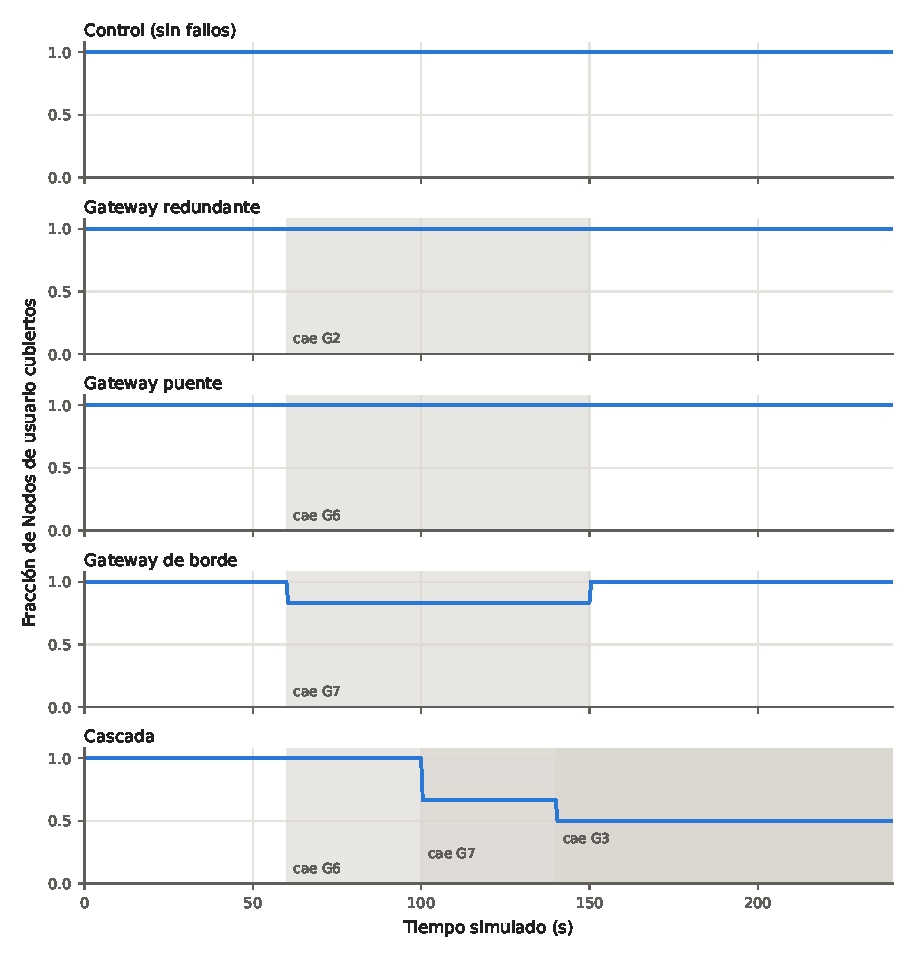
\includegraphics[width=\textwidth]{Images/Cap5/cobertura_tiempo.pdf}
    \caption{Cobertura a lo largo del tiempo en cada caso de la prueba P4. Cada panel es un caso: sin fallos, caída del Gateway redundante, del puente, del de borde y la cascada. La línea es el promedio de las 10 semillas y la banda de color, el rango entre la menor y la mayor. Las franjas grises marcan el tiempo en que hay algún Gateway caído. La cobertura solo baja en la caída de borde y en la cascada}
    \label{fig:cobertura-tiempo}
\end{figure}

\textbf{Comparación con lo calculado a mano.}
\label{sec:res-verificacion}
Tres de los resultados esperados se pueden calcular a partir del escenario, sin
simular:

\begin{itemize}
\item \textit{Caída de borde:} N6, uno de 6 usuarios, queda sin cobertura
durante 90~s de los 240~s. La cobertura media debe ser
$1 - \frac{1}{6}\cdot\frac{90}{240} = 0.9375$, donde $\frac{1}{6}$ es la
fracción de usuarios afectados y $\frac{90}{240}$ la fracción del tiempo. La
simulación da 0.938.
\item \textit{Cascada:} hay 6 usuarios cubiertos durante 100~s, 4 durante 40~s y
3 durante 100~s. La cobertura media debe ser
$\frac{6\cdot100 + 4\cdot40 + 3\cdot100}{6\cdot240} = 0.736$, es decir, los
usuarios cubiertos en cada tramo por su duración, sobre el total de usuarios por
el total de tiempo. La simulación da 0.736, con 3 usuarios cubiertos al final.
\item \textit{Puente:} la malla debe estar partida exactamente mientras G6 está
caído, 90~s, sin diferencia entre semillas. La simulación da 90.0.
\end{itemize}

Los tres coinciden. Estas comparaciones validan la forma de contar de las
métricas físicas; no dicen nada sobre el protocolo.

\textbf{La cobertura no muestra la partición.} Es el primer resultado
importante: la caída del puente mantiene la malla partida los 90~s que dura y,
sin embargo, la cobertura media es de 1.000, porque cada parte conserva algún
Gateway. En cambio, la caída de borde no parte la malla y sí reduce la
cobertura, a 0.938. Las dos métricas miden daños distintos, y un reporte basado
en una sola de ellas daría una imagen falsa del fallo. La
Figura~\ref{fig:interfaz} muestra precisamente ese estado.

\textbf{Tiempo de adaptación de las rutas.} Cuando vuelve un Gateway, las rutas
tardan 7.7~$\pm$~3.7~s en rehacerse si se cayó uno redundante, y
19.4~$\pm$~6.7~s si se cayó el puente, porque en ese caso hay que restablecer
rutas entre dos partes que estuvieron separadas
(Figura~\ref{fig:comparacion-fallos}). En la cascada no aplica, porque ningún
nodo vuelve.

\begin{figure}[htbp!]
    \centering
    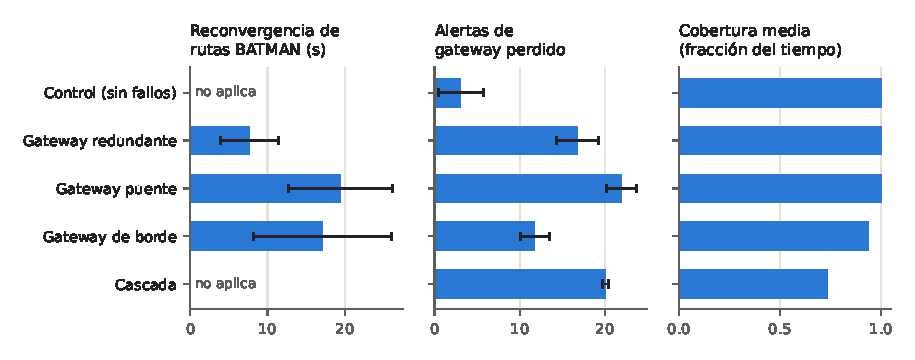
\includegraphics[width=\textwidth]{Images/Cap5/comparacion_fallos.pdf}
    \caption{Comparación de los cinco casos de la prueba P4 en tres métricas, una por panel: tiempo que tardan las rutas en rehacerse, número de alertas de Gateway perdido y cobertura media. Cada barra es el promedio de 10 semillas y la línea negra, la desviación estándar. ``No aplica'' indica que en ese caso no hubo un episodio que medir}
    \label{fig:comparacion-fallos}
\end{figure}

\textbf{Detección y falsas alarmas.} Los Gateway detectan las caídas sin
coordinador, pero con ruido. La primera alerta llega a los 72.5~$\pm$~9.2~s con
la caída del puente y a los 78.0~$\pm$~12.7~s con la del Gateway redundante, es
decir, menos de 30~s después de la caída: el tiempo límite se cuenta desde el
último mensaje oído, y en enlaces con pérdidas ya venía acumulado algo de
silencio. El caso sin fallos muestra el costo de esa sensibilidad: hay
3.1~$\pm$~2.6 alertas falsas. Con enlaces de fiabilidad entre 0.41 y 0.65, un
tiempo límite de 30~s produce falsas alarmas de vez en cuando. Es un compromiso
que la herramienta permite explorar cambiando un solo parámetro.

\textbf{Calidad de las rutas.} La Tabla~\ref{tab:cap5-calidad} indica que el TQ
medio es parecido en todos los casos, entre 0.32 y 0.36. Es un valor bajo porque
el TQ se multiplica en cada salto, sobre enlaces de fiabilidad media y rutas de
casi 3 saltos. Que suba un poco con los fallos más graves no es una mejora: al
perderse nodos desaparecen del promedio las rutas más largas, que son las de
peor TQ.

% Generado por python -m analysis.capitulo5 (no editar a mano).
\begin{table}[htbp!]
    \centering
    \caption{Calidad de las rutas y del medio en los experimentos de fallo}
    \label{tab:cap5-calidad}
    \footnotesize
    \setlength{\tabcolsep}{3pt}
    \begin{tabular}{|>{\raggedright\arraybackslash\hspace{0pt}}p{3.2cm}|>{\raggedright\arraybackslash\hspace{0pt}}p{2.8cm}|>{\raggedright\arraybackslash\hspace{0pt}}p{2.8cm}|>{\raggedright\arraybackslash\hspace{0pt}}p{2.8cm}|}
        \hline
        \textbf{Experimento} & \textbf{TQ medio de rutas} & \textbf{Saltos medios por ruta} & \textbf{Tasa de entrega del radio} \\
        \hline
        Control (sin fallos) & 0.331 $\pm$ 0.005 & 2.82 $\pm$ 0.03 & 0.600 $\pm$ 0.002 \\
        \hline
        Gateway redundante & 0.323 $\pm$ 0.004 & 2.84 $\pm$ 0.02 & 0.606 $\pm$ 0.003 \\
        \hline
        Gateway puente & 0.339 $\pm$ 0.007 & 2.85 $\pm$ 0.03 & 0.603 $\pm$ 0.003 \\
        \hline
        Gateway de borde & 0.340 $\pm$ 0.007 & 2.81 $\pm$ 0.04 & 0.599 $\pm$ 0.002 \\
        \hline
        Cascada & 0.359 $\pm$ 0.010 & 2.87 $\pm$ 0.04 & 0.601 $\pm$ 0.003 \\
        \hline
    \end{tabular}
\end{table}


\section{Los mismos fallos con Gateway móviles (prueba P5)}
\label{sec:res-fallos-movil}

Se esperaba que, si los Gateway pueden moverse, la malla pasara menos tiempo
partida. Las Tablas~\ref{tab:cap5-fallos-movil} y~\ref{tab:cap5-calidad-movil}
repiten los casos anteriores con el movimiento descentralizado.

% Generado por python -m analysis.capitulo5 (no editar a mano).
\begin{table}[htbp!]
    \centering
    \caption{Respuesta de la malla a cada fallo con Gateway móviles (descentralizada)}
    \label{tab:cap5-fallos-movil}
    \footnotesize
    \setlength{\tabcolsep}{3pt}
    \begin{tabular}{|>{\raggedright\arraybackslash\hspace{0pt}}p{2.9cm}|>{\raggedright\arraybackslash\hspace{0pt}}p{1.7cm}|>{\raggedright\arraybackslash\hspace{0pt}}p{2.6cm}|>{\raggedright\arraybackslash\hspace{0pt}}p{1.9cm}|>{\raggedright\arraybackslash\hspace{0pt}}p{2.2cm}|>{\raggedright\arraybackslash\hspace{0pt}}p{1.7cm}|}
        \hline
        \textbf{Experimento} & \textbf{Malla partida (s)} & \textbf{Reconvergencia de rutas (s)} & \textbf{Alertas} & \textbf{Cobertura media} & \textbf{Nodos cubiertos al final} \\
        \hline
        Control (sin fallos) & 0.0 & no aplica & 6.6 $\pm$ 5.6 & 1.000 & 6 \\
        \hline
        Gateway redundante & 0.0 & 15.5 $\pm$ 9.5 & 14.5 $\pm$ 2.9 & 1.000 $\pm$ 0.001 & 6 \\
        \hline
        Gateway puente & 6.2 $\pm$ 6.4 & 9.7 $\pm$ 7.0 & 14.3 $\pm$ 2.7 & 0.922 $\pm$ 0.043 & 6 $\pm$ 0 \\
        \hline
        Gateway de borde & 17.0 $\pm$ 53.8 & 30.1 $\pm$ 25.5 & 18.3 $\pm$ 7.7 & 0.959 $\pm$ 0.024 & 6 \\
        \hline
        Cascada & 6.2 $\pm$ 6.4 & 4.3 $\pm$ 4.0 & 17.2 $\pm$ 2.8 & 0.826 $\pm$ 0.054 & 4 $\pm$ 1 \\
        \hline
    \end{tabular}

    \vspace{0.4em}\parbox{14.2cm}{\scriptsize Media $\pm$ desviación estándar muestral de 10 corridas de 240 s simulados (semillas 1 a 10); sin $\pm$, la desviación es 0. ``No aplica'': ningún episodio de reconvergencia se cerró.}
\end{table}


% Generado por python -m analysis.capitulo5 (no editar a mano).
\begin{table}[htbp!]
    \centering
    \caption{Calidad de las rutas y del medio en los experimentos de fallo con Gateway móviles (descentralizada)}
    \label{tab:cap5-calidad-movil}
    \footnotesize
    \setlength{\tabcolsep}{3pt}
    \begin{tabular}{|>{\raggedright\arraybackslash\hspace{0pt}}p{3.2cm}|>{\raggedright\arraybackslash\hspace{0pt}}p{2.8cm}|>{\raggedright\arraybackslash\hspace{0pt}}p{2.8cm}|>{\raggedright\arraybackslash\hspace{0pt}}p{2.8cm}|}
        \hline
        \textbf{Experimento} & \textbf{TQ medio de rutas} & \textbf{Saltos medios por ruta} & \textbf{Tasa de entrega del radio} \\
        \hline
        Control (sin fallos) & 0.337 $\pm$ 0.010 & 2.82 $\pm$ 0.04 & 0.605 $\pm$ 0.006 \\
        \hline
        Gateway redundante & 0.348 $\pm$ 0.011 & 2.77 $\pm$ 0.03 & 0.603 $\pm$ 0.004 \\
        \hline
        Gateway puente & 0.361 $\pm$ 0.011 & 2.76 $\pm$ 0.05 & 0.597 $\pm$ 0.006 \\
        \hline
        Gateway de borde & 0.346 $\pm$ 0.010 & 2.81 $\pm$ 0.05 & 0.603 $\pm$ 0.006 \\
        \hline
        Cascada & 0.364 $\pm$ 0.009 & 2.76 $\pm$ 0.05 & 0.599 $\pm$ 0.007 \\
        \hline
    \end{tabular}
\end{table}


\textbf{La malla se adapta sola, con costos.} Sin ninguna orden central, los
Gateway que quedan se reubican. La partición por la caída del puente baja de
90~s a 6.2~$\pm$~6.4~s, y la cascada deja 4~$\pm$~1 usuarios cubiertos y una
cobertura de 0.826, frente a 3 y 0.736 con Gateway fijos. La prueba se cumple.
Pero moverse también cuesta. En la caída del puente la cobertura baja de 1.000
a 0.922~$\pm$~0.043, y en la del Gateway redundante el tiempo de adaptación de
las rutas se duplica, de 7.7~s a 15.5~$\pm$~9.5~s, porque la red sigue cambiando
mientras se rehacen las rutas. El caso sin fallos también tiene más alertas (6.6
frente a 3.1). No es una mejora en todo, sino un intercambio entre
conectividad, cobertura y estabilidad.

Una observación sobre la dispersión: en la caída de borde, el tiempo con la
malla partida es de 17.0~$\pm$~53.8~s. Ese promedio lo produce una sola semilla
entre diez; no conviene leerlo como el comportamiento típico.

\section{Modos de movimiento (pruebas P6 y P7)}
\label{sec:res-movilidad}

\textbf{P6, sin tráfico.} Se esperaba que el movimiento descentralizado
mantuviera la malla unida con una cobertura cercana a la de los modos
centralizados. La Tabla~\ref{tab:cap5-movilidad} y la Figura~\ref{fig:movilidad}
comparan los tres modos.

% Generado por python -m analysis.capitulo5 (no editar a mano).
\begin{table}[htbp!]
    \centering
    \caption{Movilidad de los Gateway: \emph{seguir}, \emph{repartir} y \emph{descentralizada}}
    \label{tab:cap5-movilidad}
    \footnotesize
    \setlength{\tabcolsep}{3pt}
    \begin{tabular}{|>{\raggedright\arraybackslash\hspace{0pt}}p{2.85cm}|>{\raggedright\arraybackslash\hspace{0pt}}p{2.5cm}|>{\raggedright\arraybackslash\hspace{0pt}}p{1.9cm}|>{\raggedright\arraybackslash\hspace{0pt}}p{1.6cm}|>{\raggedright\arraybackslash\hspace{0pt}}p{1.4cm}|>{\raggedright\arraybackslash\hspace{0pt}}p{1.9cm}|>{\raggedright\arraybackslash\hspace{0pt}}p{1.9cm}|}
        \hline
        \textbf{Escenario} & \textbf{Movilidad} & \textbf{Cobertura media} & \textbf{Componentes al final} & \textbf{Malla partida (s)} & \textbf{Entrega del radio} & \textbf{TQ medio} \\
        \hline
        base & seguir & 0.40 $\pm$ 0.19 & 1.1 $\pm$ 0.3 & 16 $\pm$ 52 & 0.86 $\pm$ 0.03 & 0.89 $\pm$ 0.03 \\
        \hline
        base & repartir & 0.95 $\pm$ 0.00 & 3.0 & 178 $\pm$ 1 & 0.49 $\pm$ 0.01 & 0.77 $\pm$ 0.03 \\
        \hline
        base & descentralizada & 0.84 $\pm$ 0.11 & 1.0 & 5 $\pm$ 15 & 0.27 $\pm$ 0.01 & 0.47 $\pm$ 0.04 \\
        \hline
        colapso\_progresivo & seguir & 0.36 $\pm$ 0.07 & 1.0 & 5 $\pm$ 15 & 0.80 $\pm$ 0.02 & 0.86 $\pm$ 0.03 \\
        \hline
        colapso\_progresivo & repartir & 0.82 $\pm$ 0.00 & 1.0 & 102 $\pm$ 1 & 0.47 $\pm$ 0.02 & 0.75 $\pm$ 0.03 \\
        \hline
        colapso\_progresivo & descentralizada & 0.42 $\pm$ 0.06 & 1.0 & 0 & 0.27 $\pm$ 0.02 & 0.51 $\pm$ 0.05 \\
        \hline
        particion & seguir & 0.67 & 2.0 & 200 & 0.96 $\pm$ 0.01 & 0.98 $\pm$ 0.01 \\
        \hline
        particion & repartir & 0.99 $\pm$ 0.00 & 3.0 & 200 & 0.79 $\pm$ 0.02 & 0.88 $\pm$ 0.02 \\
        \hline
        particion & descentralizada & 0.77 $\pm$ 0.13 & 1.8 $\pm$ 0.4 & 195 $\pm$ 12 & 0.47 $\pm$ 0.04 & 0.55 $\pm$ 0.05 \\
        \hline
        rescatista\_perdido & seguir & 0.91 $\pm$ 0.01 & 2.0 & 159 $\pm$ 0 & 0.74 $\pm$ 0.06 & 0.79 $\pm$ 0.03 \\
        \hline
        rescatista\_perdido & repartir & 0.93 $\pm$ 0.00 & 2.0 & 159 $\pm$ 0 & 0.48 $\pm$ 0.01 & 0.70 $\pm$ 0.02 \\
        \hline
        rescatista\_perdido & descentralizada & 0.75 $\pm$ 0.08 & 1.1 $\pm$ 0.3 & 59 $\pm$ 17 & 0.29 $\pm$ 0.02 & 0.56 $\pm$ 0.03 \\
        \hline
        denso & seguir & 0.51 $\pm$ 0.07 & 1.0 & 0 & 0.76 $\pm$ 0.03 & 0.82 $\pm$ 0.02 \\
        \hline
        denso & repartir & 0.99 $\pm$ 0.00 & 1.7 $\pm$ 0.5 & 85 $\pm$ 53 & 0.35 $\pm$ 0.02 & 0.50 $\pm$ 0.05 \\
        \hline
        denso & descentralizada & 0.99 $\pm$ 0.01 & 1.0 & 0 & 0.30 $\pm$ 0.00 & 0.38 $\pm$ 0.01 \\
        \hline
    \end{tabular}

    \vspace{0.4em}\parbox{15.5cm}{\scriptsize Media $\pm$ desviación estándar de 10 corridas de 200 s simulados (lote \texttt{lotes/movilidad.json}). \emph{seguir} y \emph{repartir} son la línea base centralizada; \emph{descentralizada} decide cada Gateway solo con lo que oye.}
\end{table}


\begin{figure}[htbp!]
    \centering
    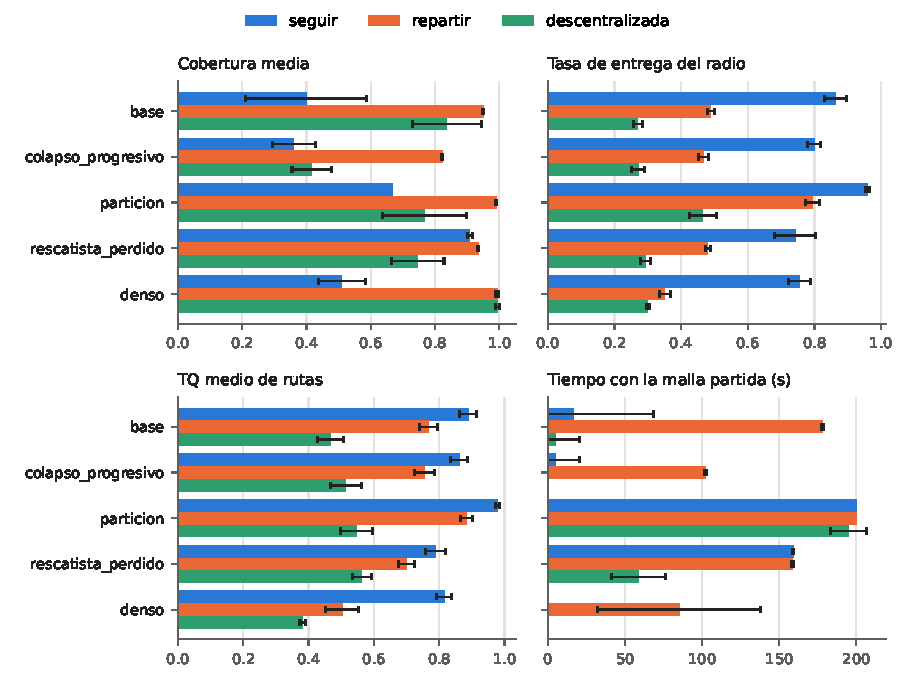
\includegraphics[width=\textwidth]{Images/Cap5/movilidad.pdf}
    \caption{Comparación de los tres modos de movimiento de los Gateway (\textit{seguir}, \textit{repartir} y descentralizado) en los cinco escenarios de la prueba P6. Cada panel es una métrica: cobertura media, tasa de entrega del radio, TQ medio de las rutas y tiempo con la malla partida. Cada barra es el promedio de 10 semillas. Ningún modo es el mejor en las cuatro métricas a la vez}
    \label{fig:movilidad}
\end{figure}

Los resultados muestran el defecto de cada regla centralizada. Con
\textit{seguir}, los Gateway se amontonan: la entrega del radio es alta porque
los enlaces son cortos, pero la cobertura es baja (0.40 en \texttt{base}, 0.51
en \texttt{denso}). Con \textit{repartir} la cobertura es casi total, pero la
malla pasa partida casi toda la corrida (178~s de 200~s en \texttt{base}). El
movimiento descentralizado queda en un punto intermedio útil: en \texttt{base}
y \texttt{denso} mantiene la malla casi siempre unida (5~s y 0~s partida) con
cobertura de 0.84 y 0.99. No gana en todo: en \texttt{colapso\_progresivo} su
cobertura (0.42) es muy inferior a la de \textit{repartir} (0.82). Y paga un
precio: el TQ y la tasa de entrega del radio son los más bajos, porque la malla
estirada usa enlaces más largos. La prueba se cumple en parte: claramente en
\texttt{base} y \texttt{denso}; en los otros tres escenarios la malla pasa menos
tiempo partida que con \textit{repartir}, pero con menos cobertura.

\textbf{P7, con tráfico.} Se esperaba que el modo que conecta a más nodos
entregara más paquetes. La Tabla~\ref{tab:cap5-movilidad-datos} y la
Figura~\ref{fig:paquetes-movilidad} añaden 6 flujos de datos.

% Generado por python -m analysis.capitulo5 (no editar a mano).
\begin{table}[htbp!]
    \centering
    \caption{Plano de datos según la movilidad de los Gateway}
    \label{tab:cap5-movilidad-datos}
    \footnotesize
    \setlength{\tabcolsep}{3pt}
    \begin{tabular}{|>{\raggedright\arraybackslash\hspace{0pt}}p{2.85cm}|>{\raggedright\arraybackslash\hspace{0pt}}p{2.5cm}|>{\raggedright\arraybackslash\hspace{0pt}}p{1.75cm}|>{\raggedright\arraybackslash\hspace{0pt}}p{1.75cm}|>{\raggedright\arraybackslash\hspace{0pt}}p{1.75cm}|>{\raggedright\arraybackslash\hspace{0pt}}p{1.75cm}|>{\raggedright\arraybackslash\hspace{0pt}}p{1.75cm}|}
        \hline
        \textbf{Escenario} & \textbf{Movilidad} & \textbf{Entrega de datos} & \textbf{Entrega con camino} & \textbf{Pérdida sin camino} & \textbf{Estiramiento} & \textbf{Exactitud del conocimiento} \\
        \hline
        base & seguir & 0.21 $\pm$ 0.13 & 0.40 $\pm$ 0.15 & 0.53 $\pm$ 0.28 & 1.04 $\pm$ 0.12 & 0.95 $\pm$ 0.02 \\
        \hline
        base & repartir & 0.20 $\pm$ 0.12 & 0.35 $\pm$ 0.13 & 0.47 $\pm$ 0.24 & 1.53 $\pm$ 0.17 & 0.90 $\pm$ 0.01 \\
        \hline
        base & descentralizada & 0.28 $\pm$ 0.15 & 0.30 $\pm$ 0.15 & 0.10 $\pm$ 0.05 & 1.03 $\pm$ 0.06 & 0.55 $\pm$ 0.05 \\
        \hline
        colapso\_progresivo & seguir & 0.22 $\pm$ 0.13 & 0.41 $\pm$ 0.15 & 0.53 $\pm$ 0.28 & 1.01 $\pm$ 0.04 & 0.94 $\pm$ 0.03 \\
        \hline
        colapso\_progresivo & repartir & 0.20 $\pm$ 0.12 & 0.33 $\pm$ 0.13 & 0.47 $\pm$ 0.24 & 1.67 $\pm$ 0.23 & 0.88 $\pm$ 0.01 \\
        \hline
        colapso\_progresivo & descentralizada & 0.23 $\pm$ 0.14 & 0.33 $\pm$ 0.16 & 0.36 $\pm$ 0.19 & 1.00 & 0.71 $\pm$ 0.07 \\
        \hline
        denso & seguir & 0.14 $\pm$ 0.08 & 0.30 $\pm$ 0.14 & 0.54 $\pm$ 0.14 & 1.20 $\pm$ 0.26 & 0.89 $\pm$ 0.06 \\
        \hline
        denso & repartir & 0.18 $\pm$ 0.09 & 0.28 $\pm$ 0.08 & 0.38 $\pm$ 0.20 & 1.41 $\pm$ 0.18 & 0.82 $\pm$ 0.07 \\
        \hline
        denso & descentralizada & 0.28 $\pm$ 0.07 & 0.28 $\pm$ 0.07 & 0.01 $\pm$ 0.01 & 1.32 $\pm$ 0.25 & 0.86 $\pm$ 0.03 \\
        \hline
    \end{tabular}

    \vspace{0.4em}\parbox{15.5cm}{\scriptsize Media $\pm$ desviación estándar de 10 corridas de 200 s con 6 flujos de datos aleatorios (lote \texttt{lotes/movilidad\_datos.json}).}
\end{table}


\begin{figure}[htbp!]
    \centering
    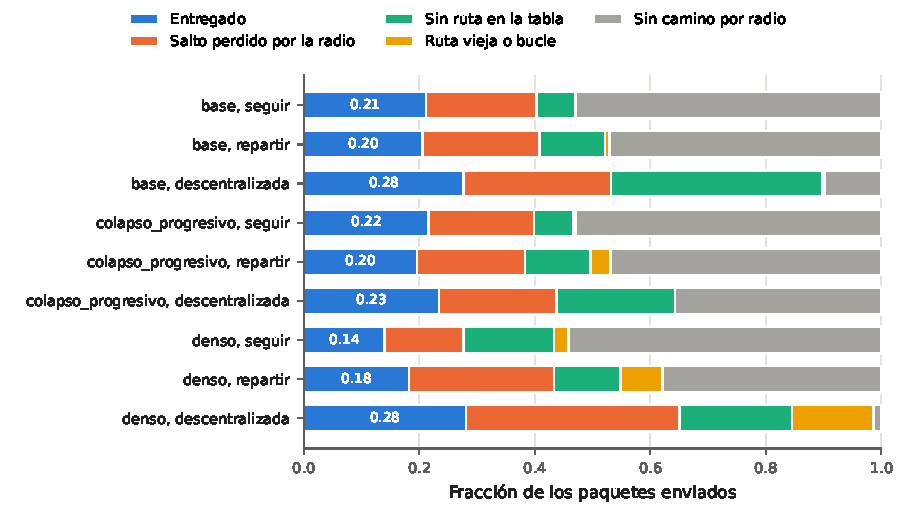
\includegraphics[width=\textwidth]{Images/Cap5/paquetes_movilidad.pdf}
    \caption{Qué pasó con los paquetes enviados en la prueba P7, según el escenario y el modo de movimiento. Cada barra representa todos los paquetes enviados (suma 1) y se divide en cinco partes: entregados, perdidos por el radio en algún salto, perdidos porque un nodo no tenía ruta, perdidos por una ruta vieja o un bucle, y sin ningún camino por radio. El modo descentralizado reduce sobre todo la parte gris (sin camino), pero aumenta las pérdidas por el radio y por falta de ruta}
    \label{fig:paquetes-movilidad}
\end{figure}

Según la Tabla~\ref{tab:cap5-diferencias}, el movimiento descentralizado
entrega más datos que \textit{repartir} en los tres escenarios, y más que
\textit{seguir} en \texttt{base} y \texttt{denso}. En
\texttt{colapso\_progresivo}, la diferencia con \textit{seguir} no es
concluyente: el intervalo incluye el cero. Las entregas son bajas en todos los
casos, entre 0.14 y 0.28. De dónde sale la ganancia también enseña algo: el
movimiento descentralizado reduce sobre todo los paquetes sin ningún camino por
radio, pero aumenta los perdidos sin ruta y por el radio. Entre los pares que sí
tienen camino, entrega menos que \textit{seguir} en \texttt{base} ($-0.104$) y
sin diferencia concluyente en los otros dos. Gana porque conecta a más pares,
no porque lleve mejor los paquetes. La prueba se cumple.

\textbf{Las tablas de rutas se quedan atrás.} Este es el costo más revelador,
y solo se ve con las métricas de lo que cree cada nodo. En \texttt{base}, la
exactitud del conocimiento baja de 0.95 con \textit{seguir} a 0.55 con el
movimiento descentralizado: en un 44~\% de los pares, el radio los conecta pero
el nodo no tiene una ruta vigente. La malla que el movimiento logra mantener
unida es tan débil que los OGM no alcanzan a mantener las rutas. Una métrica de
conectividad física diría que la red está mejor, cuando lo que hay es una red
conectada que no se conoce a sí misma. Esto sugiere ajustar el movimiento para
que tenga en cuenta la calidad de los enlaces y no solo el alcance.

\section{Fallos al azar y fallos dirigidos (prueba P8)}
\label{sec:res-robustez}

Se esperaba que dos caídas dirigidas al nodo más crítico hicieran más daño que
dos caídas al azar. La Tabla~\ref{tab:cap5-robustez} las compara.

% Generado por python -m analysis.capitulo5 (no editar a mano).
\begin{table}[htbp!]
    \centering
    \caption{Dos caídas al azar contra dos caídas dirigidas al nodo más crítico}
    \label{tab:cap5-robustez}
    \footnotesize
    \setlength{\tabcolsep}{3pt}
    \begin{tabular}{|>{\raggedright\arraybackslash\hspace{0pt}}p{2.8cm}|>{\raggedright\arraybackslash\hspace{0pt}}p{2.1cm}|>{\raggedright\arraybackslash\hspace{0pt}}p{2.2cm}|>{\raggedright\arraybackslash\hspace{0pt}}p{2.2cm}|>{\raggedright\arraybackslash\hspace{0pt}}p{2.2cm}|>{\raggedright\arraybackslash\hspace{0pt}}p{2.0cm}|}
        \hline
        \textbf{Experimento} & \textbf{Malla partida (s)} & \textbf{Entrega de datos} & \textbf{Entrega con camino} & \textbf{Cobertura media} & \textbf{Rutas fantasma} \\
        \hline
        Fallos al azar & 42 $\pm$ 57 & 0.502 $\pm$ 0.114 & 0.686 $\pm$ 0.069 & 0.925 $\pm$ 0.067 & 0.020 $\pm$ 0.013 \\
        \hline
        Fallos dirigidos & 180 & 0.284 $\pm$ 0.088 & 0.696 $\pm$ 0.087 & 0.917 & 0.052 $\pm$ 0.003 \\
        \hline
    \end{tabular}

    \vspace{0.4em}\parbox{14.7cm}{\scriptsize Media $\pm$ desviación estándar de 10 corridas de 240 s con 6 flujos de datos, caídas a los 60 y 120 s (lote \texttt{lotes/robustez.json}).}
\end{table}


Los fallos dirigidos parten la malla durante 180~s en todas las semillas,
frente a 42~$\pm$~57~s al azar, y dejan la entrega de datos en 0.284 frente a
0.502, una diferencia pareada de 0.218 (IC~95~\%: 0.149 a 0.287). La prueba se
cumple. Recuerda la distinción clásica entre errores y
ataques~\cite{Albert2000ErrorAttack}, aunque ese resultado se refiere a redes
de otro tipo y esta es una malla pequeña, de modo que es una analogía y no una
confirmación. Lo importante es lo que \textit{no} cambia: la cobertura media
(0.925 y 0.917) no distingue los dos casos, con un intervalo que incluye el
cero, porque cada parte conserva algún Gateway. Tampoco cambia la entrega entre
pares con camino (0.686 y 0.696): el enrutamiento sigue funcionando dentro de
cada parte, y el daño es la falta de camino, que explica el 59.9~\% de los
paquetes en los fallos dirigidos. Sin paquetes de datos, este daño no se habría
visto con la métrica de cobertura.

\section{B.A.T.M.A.N. e inundación (prueba P9)}
\label{sec:res-generalidad}

Se esperaba que la inundación entregara más que B.A.T.M.A.N. a cambio de más
transmisiones. La Tabla~\ref{tab:cap5-generalidad} y la
Figura~\ref{fig:paquetes-comparacion} comparan los dos protocolos en dos mapas.

% Generado por python -m analysis.capitulo5 (no editar a mano).
\begin{table}[htbp!]
    \centering
    \caption{B.A.T.M.A.N. contra inundación en dos mapas}
    \label{tab:cap5-generalidad}
    \footnotesize
    \setlength{\tabcolsep}{3pt}
    \begin{tabular}{|>{\raggedright\arraybackslash\hspace{0pt}}p{3.3cm}|>{\raggedright\arraybackslash\hspace{0pt}}p{2.2cm}|>{\raggedright\arraybackslash\hspace{0pt}}p{2.1cm}|>{\raggedright\arraybackslash\hspace{0pt}}p{2.1cm}|>{\raggedright\arraybackslash\hspace{0pt}}p{2.1cm}|>{\raggedright\arraybackslash\hspace{0pt}}p{1.6cm}|}
        \hline
        \textbf{Entorno} & \textbf{Protocolo} & \textbf{Entrega de datos} & \textbf{Entrega con camino} & \textbf{Transmisiones por paquete} & \textbf{Saltos} \\
        \hline
        Campo abierto, usuarios en grupos & B.A.T.M.A.N. & 0.575 $\pm$ 0.128 & 0.803 $\pm$ 0.090 & 2.86 $\pm$ 0.91 & 1.55 $\pm$ 0.21 \\
        \hline
        Campo abierto, usuarios en grupos & Inundación & 0.607 $\pm$ 0.127 & 0.937 $\pm$ 0.042 & 5.62 $\pm$ 1.38 & 1.56 $\pm$ 0.20 \\
        \hline
        Campo abierto, random waypoint & B.A.T.M.A.N. & 0.446 $\pm$ 0.064 & 0.544 $\pm$ 0.078 & 3.38 $\pm$ 1.08 & 1.79 $\pm$ 0.23 \\
        \hline
        Campo abierto, random waypoint & Inundación & 0.618 $\pm$ 0.063 & 0.743 $\pm$ 0.071 & 7.40 $\pm$ 1.27 & 2.24 $\pm$ 0.29 \\
        \hline
        Edificio, nodos fijos & B.A.T.M.A.N. & 0.786 $\pm$ 0.054 & 0.786 $\pm$ 0.054 & 7.19 $\pm$ 1.73 & 3.90 $\pm$ 0.74 \\
        \hline
        Edificio, nodos fijos & Inundación & 0.430 $\pm$ 0.081 & 0.430 $\pm$ 0.081 & 6.96 $\pm$ 0.34 & 4.30 $\pm$ 0.78 \\
        \hline
    \end{tabular}

    \vspace{0.4em}\parbox{14.6cm}{\scriptsize Media $\pm$ desviación estándar de 10 corridas de 300 s (lote \texttt{lotes/generalidad.json}). B.A.T.M.A.N. reintenta cada salto hasta 3 veces (unicast); la inundación difunde una vez, sin reintentos.}
\end{table}


\begin{figure}[htbp!]
    \centering
    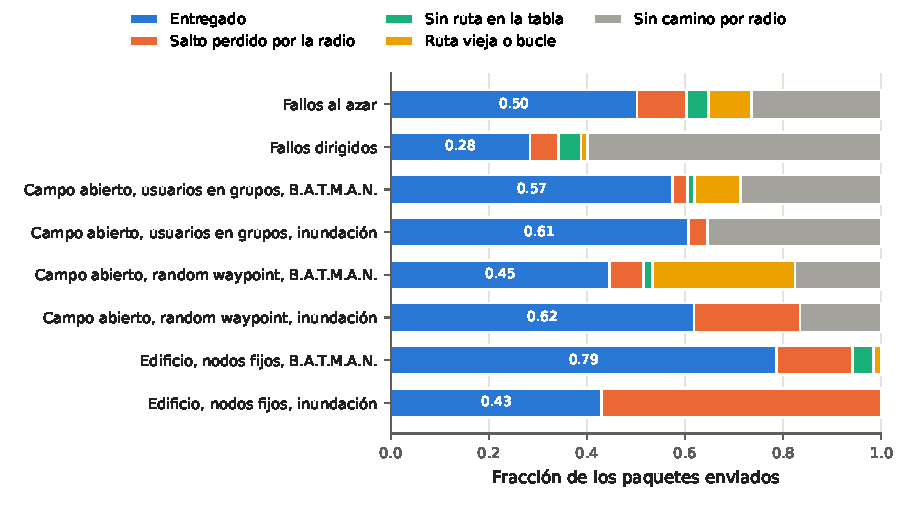
\includegraphics[width=\textwidth]{Images/Cap5/paquetes_comparacion.pdf}
    \caption{Qué pasó con los paquetes enviados en las pruebas P8 (fallos al azar y dirigidos) y P9 (B.A.T.M.A.N. e inundación en campo abierto y en el edificio). Cada barra representa todos los paquetes enviados y se divide en las mismas cinco partes de la Figura~\ref{fig:paquetes-movilidad}. En los fallos dirigidos domina la parte gris (sin camino por radio); en el edificio, la inundación pierde la mayoría de los paquetes por el radio}
    \label{fig:paquetes-comparacion}
\end{figure}

La respuesta depende del lugar, y esta es una razón para no atar un simulador a
un solo mapa. En campo abierto se cumple lo esperado: la inundación entrega más
que B.A.T.M.A.N. entre pares con camino (0.937 frente a 0.803 con usuarios en
grupos; 0.743 frente a 0.544 con usuarios que caminan al azar), con cerca del
doble de transmisiones por paquete. Cuando los usuarios se mueven al azar, la
causa principal de pérdida de B.A.T.M.A.N. es la ruta vieja (27.6~\% de los
paquetes): las tablas no siguen el ritmo del movimiento. En el edificio ocurre
lo contrario y la prueba no se cumple: B.A.T.M.A.N. entrega 0.786 frente a 0.430
de la inundación, con un número de transmisiones parecido (7.19 y 6.96). Allí
las rutas son largas (casi 4 saltos) sobre enlaces de fiabilidad media;
B.A.T.M.A.N. reintenta cada salto hasta tres veces y la inundación no, por lo
que sus copias se van perdiendo por el camino.

Hay dos precauciones. Primero, las transmisiones por paquete solo cuentan los
datos, no los OGM que B.A.T.M.A.N. necesita y la inundación no. Segundo, el
medio no representa colisiones, de modo que no refleja el principal costo
conocido de la inundación, que es saturar el
medio~\cite{Ni1999BroadcastStorm}. Los dos sesgos van en sentidos contrarios, y
la comparación vale para la entrega dentro de este modelo, no como un veredicto
sobre los protocolos.

La Tabla~\ref{tab:cap5-diferencias} reúne las diferencias pareadas de las
pruebas P7, P8 y P9.

% Generado por python -m analysis.capitulo5 (no editar a mano).
\begin{table}[htbp!]
    \centering
    \caption{Diferencias pareadas por semilla, con intervalo de confianza del 95~\%}
    \label{tab:cap5-diferencias}
    \footnotesize
    \setlength{\tabcolsep}{3pt}
    \begin{tabular}{|>{\raggedright\arraybackslash\hspace{0pt}}p{7.2cm}|>{\raggedright\arraybackslash\hspace{0pt}}p{1.9cm}|>{\raggedright\arraybackslash\hspace{0pt}}p{3.0cm}|>{\raggedright\arraybackslash\hspace{0pt}}p{1.5cm}|}
        \hline
        \textbf{Comparación} & \textbf{Diferencia media} & \textbf{Intervalo del 95~\%} & \textbf{¿Excluye el 0?} \\
        \hline
        base: entrega, descentralizada $-$ seguir & +0.065 & [+0.020, +0.111] & sí \\
        \hline
        base: entrega, descentralizada $-$ repartir & +0.072 & [+0.032, +0.111] & sí \\
        \hline
        base: entrega con camino, descentralizada $-$ seguir & $-$0.104 & [$-$0.195, $-$0.014] & sí \\
        \hline
        colapso\_progresivo: entrega, descentralizada $-$ seguir & +0.018 & [$-$0.016, +0.052] & no \\
        \hline
        colapso\_progresivo: entrega, descentralizada $-$ repartir & +0.038 & [+0.018, +0.058] & sí \\
        \hline
        colapso\_progresivo: entrega con camino, descentralizada $-$ seguir & $-$0.080 & [$-$0.166, +0.005] & no \\
        \hline
        denso: entrega, descentralizada $-$ seguir & +0.141 & [+0.106, +0.176] & sí \\
        \hline
        denso: entrega, descentralizada $-$ repartir & +0.099 & [+0.060, +0.138] & sí \\
        \hline
        denso: entrega con camino, descentralizada $-$ seguir & $-$0.012 & [$-$0.083, +0.060] & no \\
        \hline
        Robustez: entrega, azar $-$ dirigida & +0.218 & [+0.149, +0.287] & sí \\
        \hline
        Robustez: cobertura, azar $-$ dirigida & +0.008 & [$-$0.040, +0.057] & no \\
        \hline
        Campo abierto, usuarios en grupos: entrega con camino, inundación $-$ B.A.T.M.A.N. & +0.134 & [+0.067, +0.202] & sí \\
        \hline
        Campo abierto, random waypoint: entrega con camino, inundación $-$ B.A.T.M.A.N. & +0.199 & [+0.114, +0.284] & sí \\
        \hline
        Edificio, nodos fijos: entrega con camino, inundación $-$ B.A.T.M.A.N. & $-$0.356 & [$-$0.388, $-$0.325] & sí \\
        \hline
    \end{tabular}

    \vspace{0.4em}\parbox{14.4cm}{\scriptsize Intervalo $t$ de Student con 9 grados de libertad sobre las diferencias entre corridas con la misma semilla. Sin corrección por comparaciones múltiples.}
\end{table}


\section{Repetibilidad y tamaño de la red (pruebas P10 y P11)}
\label{sec:res-repetibilidad}

\textbf{P10, repetibilidad.} Se esperaba que la misma semilla diera la misma
corrida. El 4 de noviembre de 2026 se volvieron a correr todos los lotes en un
computador distinto de aquel en el que se habían generado las tablas el 27 de
octubre, y las cinco tablas de esos lotes salieron idénticas byte a byte. El 13
de noviembre, después de añadir los tipos de paquete, se repitieron los tres
lotes con tráfico de datos y sus tablas volvieron a salir idénticas. También
se comprobó que la interfaz web produce la misma serie de métricas que la
terminal con la misma semilla. La prueba se cumple: los resultados no solo son
parecidos, son exactamente los mismos (requerimiento R6).

\textbf{P11, tamaño de la red.} La Tabla~\ref{tab:escala} muestra que el
simulador corre más rápido que el tiempo real hasta unas decenas de nodos y más
lento a partir de unos 100 nodos juntos. Ese es su rango de uso.

\section{Lo que las pruebas mostraron sobre el protocolo}
\label{sec:res-protocolo}

Llevar los paquetes con las tablas de cada nodo dejó ver dos comportamientos
que antes no se podían observar:

\begin{itemize}
\item \textbf{Bucles.} Entre el 1.3~\% y el 2.3~\% de los paquetes se pierde
dando vueltas entre nodos, en las pruebas P8 y P9 con B.A.T.M.A.N. La causa
probable es que esta implementación reenvía la primera copia de cada OGM, en
lugar de solo la del mejor vecino, como hace el protocolo.
\item \textbf{Reparación lenta.} Cuando se cae un Gateway, la ruta que pasaba
por él permanece en las tablas cerca de 50~s (observado al examinar corridas de
la caída del Gateway redundante), porque solo se reemplaza cuando aparece otra
mejor. En la prueba de fallos al azar, el 7.4~\% de los paquetes se pierde por
este motivo. El protocolo borra al nodo de origen cuando pasa un tiempo sin
oírlo.
\item \textbf{Efecto de corregir el TQ.} Antes de la corrección, el TQ de toda
ruta valía 1.0, de modo que la medida central del protocolo no decía nada. Con
nodos fijos y la semilla 1, el TQ medio pasó a 0.740 en \texttt{base}, 0.514 en
\texttt{denso} y 0.711 en \texttt{particion}. La red parecía perfecta sin serlo.
\end{itemize}

Los dos primeros no se corrigieron, a propósito: hacerlo cambiaría el
funcionamiento del protocolo, y se prefirió reportarlos. Son el tipo de hallazgo
que justifica ejecutar el código en lugar de un modelo idealizado: una copia
escrita con la especificación en mente no los habría producido. Y, a la
inversa, marcan el límite de los resultados: parte de las pérdidas de este
capítulo pertenecen a esta implementación y no a B.A.T.M.A.N.\ en general.

\section{Resumen de las pruebas}
\label{sec:res-resumen}

\begin{table}[htbp!]
    \centering
    \caption{Resumen de las pruebas: lo que se esperaba, lo que se obtuvo y si coinciden}
    \label{tab:resumen-pruebas}
    \footnotesize
    \begin{tabular}{|p{0.6cm}|p{4.4cm}|p{6.6cm}|p{1.6cm}|}
        \hline
        \textbf{N.º} & \textbf{Qué se esperaba} & \textbf{Qué se obtuvo} & \textbf{¿Coincide?} \\
        \hline
        P1 & Casi todos los pares conectados con ruta a los 30~s & 152 de 156 pares (97~\%) & Sí \\
        \hline
        P2 & El TTL baja en uno por salto & De 6 al salir del origen a 2 tras cuatro reenvíos & Sí \\
        \hline
        P3 & ICMP $<$ UDP $<$ TCP en entrega; TCP con más transmisiones & 0.646, 0.772 y 0.924; TCP usa 2.6 veces las transmisiones de UDP & Sí \\
        \hline
        P4 & Partición de 90~s por el puente; cobertura de 0.9375 por el borde y de 0.736 en la cascada & 90.0~s; 0.938; 0.736 & Sí \\
        \hline
        P5 & Menos tiempo con la malla partida & De 90~s a 6.2~s en la caída del puente, con cobertura de 0.922 & Sí, con costo \\
        \hline
        P6 & Malla unida con cobertura cercana a la centralizada & Se logra en \texttt{base} y \texttt{denso}; en los otros tres escenarios la cobertura es menor que con \textit{repartir} & En parte \\
        \hline
        P7 & Más entrega al conectar a más nodos & Más entrega que \textit{repartir} en 3 de 3 escenarios y que \textit{seguir} en 2 de 3 & Sí \\
        \hline
        P8 & Los fallos dirigidos hacen más daño & Entrega de 0.284 frente a 0.502; la cobertura no los distingue & Sí \\
        \hline
        P9 & La inundación entrega más, con más transmisiones & Sí en campo abierto; en el edificio entrega menos (0.430 frente a 0.786) & En parte \\
        \hline
        P10 & Tablas idénticas al repetir & Idénticas byte a byte en dos computadores & Sí \\
        \hline
        P11 & El costo crece con los nodos & Más rápido que el tiempo real hasta decenas de nodos & Sí \\
        \hline
    \end{tabular}
\end{table}

\section{Discusión}
\label{sec:discusion}

La pregunta del planteamiento era cómo implementar un simulador para redes
descentralizadas que ejecute el código de los nodos, represente el medio de un
edificio, decida solo con información local y permita medir la cobertura y la
adaptabilidad. Las pruebas permiten responderla por partes.

\textbf{Qué requerimientos fueron decisivos.} Separar las pérdidas físicas de
las de enrutamiento y medir lo que cree cada nodo frente a la realidad (R5)
explica buena parte de los hallazgos de este capítulo. La regla de decidir solo
con información local (R4) no es un capricho: al aplicarla aparecieron las
tablas de rutas atrasadas y los bucles, ocultos mientras los mensajes se
entregaban por la red real. En cambio, R7 se cumple solo en parte, como muestra
la Tabla~\ref{tab:escala}.

\textbf{Cobertura.} El resultado que más se repite es que \textit{una sola
medida de conectividad oculta el daño}: la cobertura no distingue una
partición, no separa un fallo dirigido de uno al azar, y la conectividad física
no refleja que los nodos desconocen sus rutas. Para evaluar una red
descentralizada hay que medir a la vez la física, la entrega de datos y lo que
cree cada nodo.

\textbf{Adaptabilidad.} El movimiento descentralizado consigue resultados que
compiten con las reglas centralizadas sin usar información global, y permite
que la malla se adapte sola a un fallo. Sus costos son concretos: enlaces más
débiles, tablas de rutas atrasadas y más alertas. Esto es coherente con el
compromiso entre cobertura y conectividad que describe la literatura de
despliegue autónomo~\cite{Poduri2004ConstrainedCoverage}.

\textbf{Qué le falta al simulador frente a otras herramientas.} La
Tabla~\ref{tab:faltantes} compara el simulador con las herramientas revisadas
en el Capítulo~\ref{cap:estado-arte}. Lo que este trabajo aporta está en las
últimas filas; lo que le falta, en las primeras, y coincide con las
limitaciones declaradas.

\begin{table}[htbp!]
    \centering
    \caption{Comparación del simulador con las herramientas revisadas: qué ofrece cada una. Las primeras filas son lo que le falta a este simulador; las últimas, lo que aporta}
    \label{tab:faltantes}
    \footnotesize
    \begin{tabular}{|p{4.3cm}|p{2.6cm}|p{2.9cm}|p{3.3cm}|}
        \hline
        \textbf{Característica} & \textbf{ns-3 y OMNeT++/INET} & \textbf{CORE, EMANE y Mininet-WiFi} & \textbf{Este simulador} \\
        \hline
        Colisiones, interferencia y acceso al medio & Sí, con modelos detallados~\cite{Ns3Modelos,InetFramework} & Sí, con EMANE~\cite{Emane} & No \\
        \hline
        Modelos de propagación calibrados & Varios~\cite{Ns3Modelos} & Varios~\cite{Emane} & Uno, simple y sin calibrar \\
        \hline
        Retardo de los paquetes & Sí & Sí, en tiempo real & No: cada salto ocurre dentro de un paso \\
        \hline
        Pila de Internet completa (IP, TCP con congestión) & Sí~\cite{InetFramework} & Sí, la de Linux~\cite{Ahrenholz2008Core,Fontes2015MininetWifi} & No: tres tipos de paquete simplificados \\
        \hline
        Redes de cientos de nodos & Sí & Más de cien~\cite{Ahrenholz2008Core} & Decenas \\
        \hline
        Ejecutar el código del nodo sin reescribirlo & Solo con \textit{Direct Code Execution}~\cite{Tazaki2013DCE} & Sí & Sí, las clases en Python del nodo \\
        \hline
        Modelo de pérdida entre pisos & ns-3 trae un módulo de edificios~\cite{Ns3Modelos}; hay que configurarlo & Hay que configurarlo & Sí, listo para usar \\
        \hline
        Medir lo que cree cada nodo frente a la realidad & Lo programa el usuario & Lo programa el usuario & Sí, incluido \\
        \hline
        Repetir exactamente una corrida & Sí, con semilla & Difícil: depende del tiempo real & Sí, con semilla \\
        \hline
    \end{tabular}
\end{table}

\textbf{Hasta dónde llegan estas conclusiones.} Sin una validación con equipos
físicos ni contra batman-adv, las magnitudes absolutas no se pueden trasladar a
una red real. El medio es optimista en varios
aspectos~\cite{Kotz2004Assumptions} y los umbrales del movimiento se ajustaron
sobre parte de los mismos escenarios. Los resultados más sólidos son los que
tienen una causa física clara, como el de la cobertura frente a la partición;
los más frágiles son las comparaciones de magnitud pequeña, sobre todo las
diferencias con intervalos cercanos al cero.
